\section{Introduction}

This project aims to develop an algorithm to compute a flyby of a planet in the
Solar System, with possibility of doing a gravity assist on it. The planet that will
be considered in this particular case is Jupiter, the heaviest planet in the Solar
System, meaning that is one of the best possibilities to perform a gravity assist.

The purpose of this calculation could be try to repeat the mission to Pluto that
Nasa's New Horizons mission \cite{NASA_NewHorizons} is currently doing. New Horizons
is a mission that was launched on January 19, 2006 from Cape Canaveral, Florida
with the objective of being the first spacecraft to fly-by Pluto. In order to arrive
to Pluto in a shorter period of time, New Horizons get a gravity assist on Jupiter
on February 28, 2007, a bit more than a year after leaving Earth's Sphere of Influence
with a velocity of $16.23 km s^{-1}$, in an hyperbolic solar escape trajectory.

With this work, the objective is to calculate a possible future opportunity to perform
a gravity assist on Jupiter, that could send the spacecraft again to Pluto. Given
that the orbit of Pluto has a inclination quite different from the rest of planets
in the Solar System, an easier mission would be repeating the fly-by of
Ultima Thule ($2014 MU_{69}$), instead of Pluto, that has an inclination close to
zero and also is much more circular, with an eccentricity close to zero, making easier
and cheaper the trajectory.

The code that has been developed in Python would simply calculate the next launch
windows to arrive to Jupiter by performing a single burn tangential to the Earth
orbit. The code will benefit from the power of Python library Poliastro \cite{poliastro},
which implement a collection of classes and methods that helps plotting and calculating
orbital parameters. So the purpose of this work also includes helping the user to
familiarize with the use of this library in order to perform useful calculations.

\section{Theoretical calculations}

Given that Earth and Jupiter orbits have quite similar inclination and are almost
circular, that calculations could be simplified. The eccentricity of both orbits
are:

\begin{equation*}
	e_{\oplus} = 0.022847
\end{equation*}

\begin{equation*}
	e_{\jupiter} = 0.050360
\end{equation*}

And the relative inclination is:

\begin{equation*}
	i = 0.1992^{\circ}
\end{equation*}

The next calculations would compute an orbit that crosses Jupiter orbit doing a
tangential burn at Earth with an impulsive maneuver of a given $\Delta V$. The
transit orbit we obtain could be both elliptical or hyperbolic, with the only
constraint that (if elliptical), its aphelion should be larger than the Jupiter
orbit radius. To calculate this minimum elliptical orbit, a Hohmann transfer
orbit has been calculated.

\begin{equation}
	a_t = \frac{r_{\oplus} + r_{\jupiter}}{2}
\end{equation}

\begin{equation}
	v_{p,trans} = \left( \frac{2GM_{\astrosun}}{r_{\oplus}} - \frac{GM_{\astrosun}}{a_t}  \right)
\end{equation}

Where $v_{p,trans}$ is the velocity at the perihelion of the transfer orbit,
so the velocity needed at Earth departure to start the transfer
ellipse that would arrive to Jupiter radius with minimal velocity tangent to Jupiter
orbit. In fact, due to that Earth has actually an orbital velocity, the $\Delta V$
that the spacecraft should apply is:

\begin{equation}
	\Delta V = v_{p,trans} - v_{\oplus}
\end{equation}

From this point, the upper limit $\Delta V$, is infinity, with the only technological
limit due to finite fuel that the spacecraft can loads.

Now that we have calculated the range of possible impulses, the aim is to compute
the transfer time to Pluto, in order to define the launch window possibilities.

For this we have to use the elliptical (or hyperbolic) mean motion, to calculate
the time required from the orbit perihelion to the true anomaly ($\nu$) when the
orbit crosses Jupiter orbit. For this, first of all, we need to calculate $\nu_{\jupiter}$
when the radius vector of the transfer orbit reaches the radius of Jupiter. Here
we don't have to distinguish if the orbit is elliptic or hyperbolic. Using:

\begin{equation}
	e = \frac{r_a - r_p}{r_a + r_p}
\end{equation}

\begin{equation}
	p = a_t(1-e^2)
\end{equation}

\begin{equation}
	r = \frac{p}{1 + e \cos{\nu}}
\end{equation}

it can be obtained $\nu$ when this transfer orbit crosses Jupiter.

Now, the transfer time from perihelion to $\nu_{\jupiter}$ with,
depending on the type of orbit (elliptical (a) or hyperbolic (b)):

\begin{subequations}
\begin{equation}
	\Delta t_{trans} = \frac{E_{\jupiter} - e \sin{E_{\jupiter}}}{n}
\end{equation}
\begin{equation}
	\Delta t_{trans} = \frac{e \sinh{F_{\jupiter}} - F_{\jupiter}}{n}
\end{equation}
\end{subequations}
where:

\begin{subequations}
\begin{equation}
	\cos{E_{\jupiter}} = \frac{e + \cos{\nu_{\jupiter}}}{1 + e \cos{\nu_{\jupiter}}}
\end{equation}
\begin{equation}
	\cosh{F_{\jupiter}} = \frac{e + \cos{\nu_{\jupiter}}}{1 + e \cos{\nu_{\jupiter}}} \tan{\frac{\nu_{\jupiter}}{2}}
\end{equation}
\end{subequations}

and the mean motion, $n$:

\begin{subequations}
\begin{equation}
	n = \sqrt{\frac{GM_{\astrosun}}{a_t^3}}
\end{equation}
\begin{equation}
	n = \sqrt{\frac{GM_{\astrosun}}{(-a_t)^3}}
\end{equation}
\end{subequations}

After doing that we can know where should be placed Jupiter at the launch day,
respect to the Earth in order to get to Jupiter at the exact time that Jupiter is
actually there. We simply have to subtract the angle ($\Delta \nu$) that Jupiter
would do in $\Delta t_{trans}$. For this we have assumed that Jupiter has a constant
angular velocity:
\begin{equation}
	\omega_{\jupiter} = \frac{v_{\jupiter}}{r_{\jupiter}}
\end{equation}

And now, $\nu$ of Jupiter at the time of launch from Earth would be:

\begin{equation}
	\Delta \nu_{\jupiter, launch} = \nu_{\jupiter} - \omega_{\jupiter} \Delta t_{trans}
\end{equation}

And finally, knowing the true anomaly at which Jupiter is today, we can compute
the time required to Jupiter and the Earth reach an angular separation of
$\nu_{\jupiter, launch}$, when we should launch the rocket from Earth to reach
Jupiter with the mentioned $\Delta V$.

This time until launch would be:

\begin{equation}
	t_{launch} = \frac{\Delta \nu_{today} - \Delta \nu_{\jupiter, launch}}{\omega_{\oplus} - \omega_{\jupiter}}
\end{equation}

, where $\Delta \nu_{today}$ is the difference in true anomalies between Earth
and Jupiter today, seen from the Sun.

\section{Code description}

The code, as previously mentioned was developed in Python using the astrodynamics
library \textit{poliastro}, which would help us to perform those calculations.

The function \texttt{Earth\_to\_Jupiter(dv)} gets the $\Delta V$ desired and
returns:

\begin{itemize}
	\item ss\_transfer = transfer orbit object
	\item t = time to the first next launch window
	\item T = period between launch windows
	\item t\_transfer = transfer time from Earth to Jupiter
\end{itemize}

Inside the function, a test transfer orbit (launching today) has been created in
order to calculate the \texttt{nu\_Jupiter}, ($\nu_{\jupiter, launch}$).

The interesting point of using \textit{poliastro} is that it implements a quite
comfortable way to define orbits and get its parameters.

The functions:\\
\texttt{from poliastro.bodies import Earth, Jupiter, Sun}\\
\texttt{from poliastro.twobody import Orbit}\\
\texttt{ss\_Earth = Orbit.from\_body\_ephem(Earth)}\\
\texttt{ss\_Jupiter = Orbit.from\_body\_ephem(Jupiter)}

returns the orbits of both bodies at today's date.
And the objects returned also implements functions to get all the parameters of the
orbit, like eccentricity, semi-major axis, period, radius vector, velocity...

So with this, and the implementation of some of the previous equations, the results
are computed. One point of particular interest is that the function
\texttt{nu\_to\_M(nu,ecc)} from the \texttt{poliastro.twobody.angles} module converts
true anomalies to eccentric anomalies, for both elliptic and hyperbolic orbits,
according to the eccentric (ecc) value given.

Finally, the function implements a propagator that would actually compute the time
from today to the launch date, and from the launch date to the arrival date, for
each one of the bodies involved (Earth, Jupiter and the spacecraft). This way we
can finally know the position of the bodies in each of the instants and verify if
the computations has been done correctly.

The propagator used is already implemented inside \textit{poliastro}, and it's
called using the next:
\texttt{Orbit.propagate(t)}

where Orbit is the orbit state object we want to propagate, and t, the time of
integration, that can also be negative for past moments.

Finally, the results are plotted for each time step and also the orbits of each
object.

\section{Results}

The first result that has been obtained are using the same $\Delta V$ as New Horizons
used for its first impulse: $\Delta V = 16.23 km s^{-1}$, in order to compare our
results with the one that New Horizons did. The plot that the code outputs is shown
in figure \ref{fig:NH_transfer}:

\begin{figure}[h!]
	\centering
	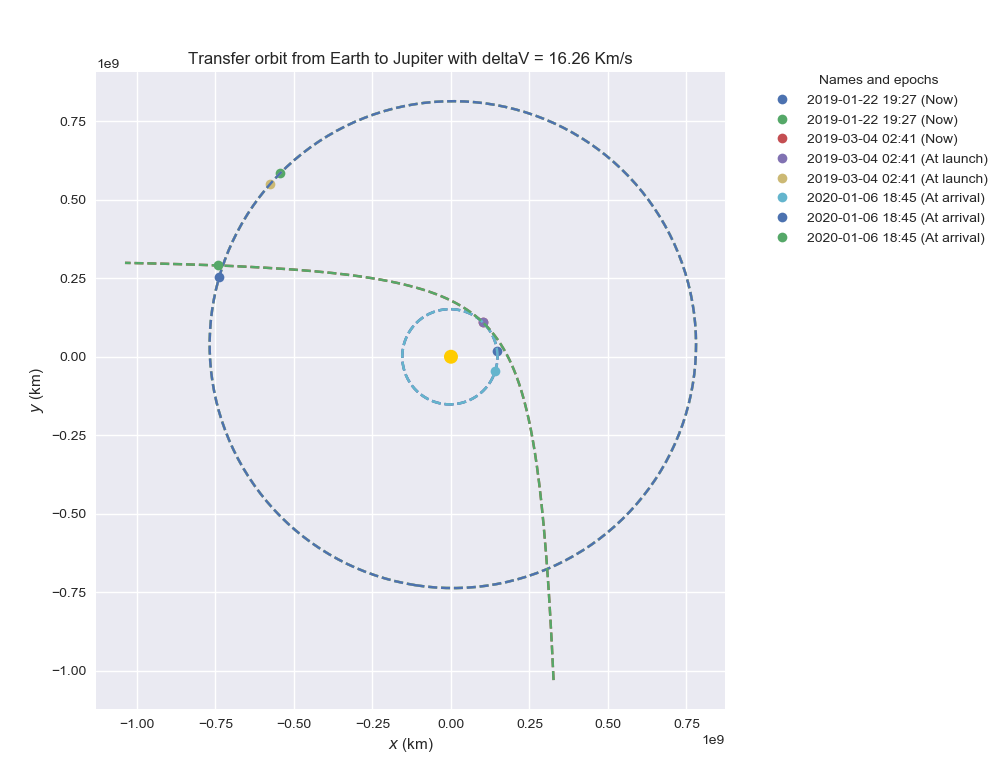
\includegraphics[width=0.8\textwidth]{img/Transfer_New_Horizons_2019.png}
	\caption{Results for New Horizons transfer from Earth to Jupiter}
	\label{fig:NH_transfer}
\end{figure}

\newpage
So, the next launch window would be next March 4th, 2019 at 2:41 UTC, and the
arrival date would be January 6th, 2020 at 18:45 UTC.

The function also gives the user the following outputs:\\
\texttt{Time from now to the next launch window = 40.121 d}\\
\texttt{Time between launch windows = 386.431 d}\\
\texttt{Transfer time from Earth to Jupiter = 308.669 d}\\

In the plot it can be seen an inaccuracy in the position of Jupiter and the spacecraft
at the arrival date. This should be due to the approximations that has been done,
like considering circular, coplanar orbits.

Finally, to see how the transfer time changes as function of $\Delta V$, the next
plot has been computed:

\begin{figure}[h]
	\centering
	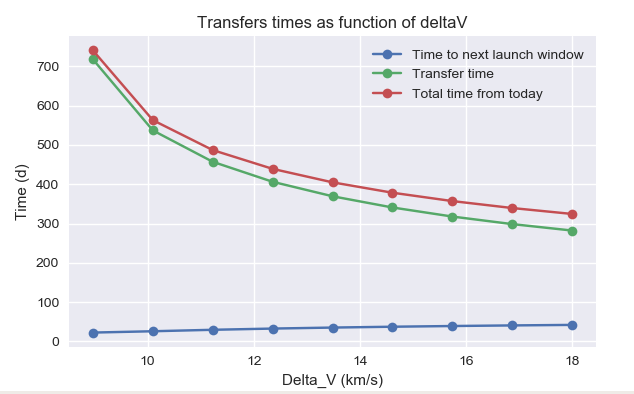
\includegraphics[width=0.8\textwidth]{img/Transfer_times.png}
	\caption{Transfer time for several values of $\Delta V$}
	\label{fig:transfer_times}
\end{figure}
